
%%%%%%%%%%%%%%%%%%%%%%%%%%%%%%%%%%%%%%%%
% Friggeri Resume/CV
% XeLaTeX Template
% Version 1.0 (5/5/13)
%
% This template has been downloaded from:
% http://www.LaTeXTemplates.com
%
% Original author:
% Adrien Friggeri (adrien@friggeri.net)
% https://github.com/afriggeri/CV
%
% License:
% CC BY-NC-SA 3.0 (http://creativecommons.org/licenses/by-nc-sa/3.0/)
%
% Important notes:
% This template needs to be compiled with XeLaTeX and the bibliography, if used,
% needs to be compiled with biber rather than bibtex.
%
%%%%%%%%%%%%%%%%%%%%%%%%%%%%%%%%%%%%%%%%%
\RequirePackage{fixltx2e}
\documentclass[]{friggeri-cv} % Add 'print' as an option into the square bracket to remove colors from this template for printing
\usepackage{color}

\addbibresource{bibliography.bib} % Specify the bibliography file to include publications

%for Fancy Quotations
\newcommand*\openquote{\makebox(25,-5){\scalebox{5}{``}}}
\newcommand*\closequote{\makebox(25,-22){\scalebox{5}{''}}}
\colorlet{shadecolor}{Azure}

\makeatletter
\newif\if@right
\def\shadequote{\@righttrue\shadequote@i}
\def\shadequote@i{\begin{snugshade}\begin{quote}\openquote}
		\def\endshadequote{%
			\if@right\hfill\fi\closequote\end{quote}\end{snugshade}}
\@namedef{shadequote*}{\@rightfalse\shadequote@i}
\@namedef{endshadequote*}{\endshadequote}
\makeatother
%End of famcy quotations
\usepackage{multirow}
\begin{document}

\header{Dr. Ritesh}{Ajoodha}{Tenure Lecturer} % Computer Scientist \& Mathematician Your name and current job title/field

%----------------------------------------------------------------------------------------
%	SIDEBAR SECTION
%----------------------------------------------------------------------------------------

\begin{aside} % In the aside, each new line forces a line break
\section{contact}
1 Jan Smuts Avenue
Braamfontein, Gauteng
South Africa
UG17 MSB
~
+27 74 418 3978
~
\href{mailto:ritesh.ajoodha@wits.ac.za}{ritesh.ajoodha@wits.ac.za}
\href{http://riteshajoodha.co.za/}{http://riteshajoodha.co.za/}
%\href{https://www.facebook.com/ritesh.ajoodha}{fb://RAjoodha}

\section{languages}
english \& afrikaans
\section{programming}
{\color{red} $\varheartsuit$} Java, TensorFlow
Python, C++, C, C\#
PHP, MatLab
JavaScript
Ruby
SQL \& HTML
\section{Typesetting}
\LaTeX, Microsoft Office

\section{Interests}
Probabilistic Graphical Models, Causation, Knowledge Representation and Reasoning, Logic, Computer Vision, Data Mining, Image Processing, Machine Learning, Spectral Analysis, Evolutionary Computation, Algorithmic Composition, Pattern Recognition. 
\end{aside}
%----------------------------------------------------------------------------------------
%	EDUCATION SECTION
%----------------------------------------------------------------------------------------

\section{education}

\begin{entrylist}
%------------------------------------------------
\entry
{2018--2019}
{Postgraduate Diploma {\normalfont in Higher Education}}
{The University of the Witwatersrand, Johannesburg}
{Specialisation in Higher Education. Honours equivalent, NQF8.}
%------------------------------------------------
\entry
{2015--2018}
{Doctor {\normalfont of Philosophy, Computer Science}}
{The University of the Witwatersrand, Johannesburg}
{\emph{THESIS TITLE:} {\it "Influence Modelling and Learning between Dynamic Bayesian Networks using Score-based Structure Learning"} \\ This thesis explores novel techniques to track influence between partially observable stochastic processes by using structure learning for Bayesian networks.}
%%------------------------------------------------
%\entry
%{2015--2017}
%{Fellowship {\normalfont Degree of Music}}
%{Trinity College, London}
%{The standard of piano performance is equivalent to the performance component on completion of a full-time postgraduate course at a conservatoire or university.}
%------------------------------------------------
\entry
{2015}
{Licentiate {\normalfont Degree of Music}}
{Trinity College, London}
{The standard of piano performance is equivalent to the performance component on completion of a full-time undergraduate course at a conservatoire or university.}
%------------------------------------------------
\entry
{2014}
{Master {\normalfont of Science, Computer Science}}
{The University of the Witwatersrand, Johannesburg}
{\emph{DISSERTATION TITLE:} {\it "Automatic Music Genre Classification"} - {\bf \color{bloodred}{with distinction}}\\ This dissertation explores novel techniques for music genre classification to improve music information retrieval and recommendation services.}
%------------------------------------------------
\entry
{2010--2013}
{Bachelor {\normalfont of Science} with Honours}
{The University of the Witwatersrand, Johannesburg}
{Specialization in Computer Science - {\bf \color{bloodred}{with distinction}} \\ \emph{RESEARCH REPORT:} {\it "Context-free Grammars, Gaussian Distributions and Genetic Algorithms in Algorithmic Music Composition"} \\ This research report explored a novel methodology to compose music using Charles Darwin's theory of evolution and natural selection.\\
{\bf Honours Coursework: } \emph{Introduction to Research Methods, Compilers, Analysis of Algorithms, Image Processing, Knowledge Representation and Reasoning, Computational Molecular Biology, Multi-agent Systems, Research Report.}\\
{\bf Computer Science Coursework: } \emph{Architecture and Networks III, Formal Languages and Automata III, Software Engineering III, Algorithms and Artificial Intelligence III, Application and Analysis of Algorithms II, Database Fundamentals II, Operating Systems II, Programming Languages II, Computer Science I.}\\
{\bf Pure Mathematics Coursework: } \emph{ Real Analysis III, Mathematical Economics III, Group Theory III, Complex Analysis III, Coding and Cryptography III, Number Theory III, Discrete Mathematics II, Linear Algebra II, Group Theory II, Advanced Analysis II,  Multi-variable Calculus II, Basic Analysis II, Calculus I, Algebra I.}
}
%------------------------------------------------
\entry
{2012}
{Associate {\normalfont Degree of Music}}
{Trinity College, London}
{\emph{PIANO RECITAL:} - {\bf \color{bloodred}{with distinction}} \\
The standard of performance is equivalent to the performance component of the first year in a full-time undergraduate course at a conservatoire or university.}
%------------------------------------------------
\entry
{2010}
{Grade 8 {\normalfont Pianoforte Examination}}
{Royal School of Music, London}
{Specialization in Piano - {\bf \color{bloodred}{with distinction}}}
%------------------------------------------------
\end{entrylist}

%----------------------------------------------------------------------------------------
%	WORK EXPERIENCE SECTION
%----------------------------------------------------------------------------------------

\section{experience}

\begin{entrylist}
%------------------------------------------------
\entry
{2017--Now}
{Associate {\normalfont Lecturer}}
{Computer Science and Applied Mathematics, The University of the Witwatersrand}
{Associate lecturer for \textit{Data Structures and Algorithms (COMS2004)} and Basic Computer Organisation (COMS1015) for electrical engineering and computer science students. Supervisor for Honours and Masters Students. 
}
%------------------------------------------------
\end{entrylist}

\begin{entrylist}
%------------------------------------------------
\entry
{2017--Now}
{Associate {\normalfont Lecturer}}
{Computer Science and Applied Mathematics, The University of the Witwatersrand}
{Associate lecturer for \textit{Data Structures and Algorithms (COMS2004)} and Basic Computer Organisation (COMS1015) for electrical engineering and computer science students. Supervisor for Honours and Masters Students. 
}
%------------------------------------------------
\entry
{2015--2016}
{Sessional {\normalfont Lecturer}}
{Computer Science and Applied Mathematics, The University of the Witwatersrand}
{Sessional lecturer for \textit{Data Structures and Algorithms (COMS2004)} and Basic Computer Organisation (COMS1015) for electrical engineering and computer science students.  
}
%------------------------------------------------
\entry
{2013--2015}
{Senior {\normalfont Tutor}}
{Computer Science, The University of the Witwatersrand}
{Developed Laboratory and other written assessments for first year computer science students. Examined and assessed students' submissions, this included marking test and assignments.}
%------------------------------------------------
\end{entrylist}

%----------------------------------------------------------------------------------------
%	AWARDS SECTION
%----------------------------------------------------------------------------------------

\section{awards and Funding}

\begin{entrylist}
%------------------------------------------------
\entry
{2018}
{Wits Staff Bursary}
{The University of the Witwatersrand}
{Valued at {\bf \color{ForestGreen}{R40 000}}. Toward the Postgraduate Diploma {\normalfont in Higher Education}.}
%------------------------------------------------
\entry
{2017}
{Teaching Development Grant (TDG)}
{University of Pretoria}
{Valued at {\bf \color{ForestGreen}{R50 000}}. This funding is for emerging staff at selected SA HEIs who are also simultaneously registered for a M/PhD. The purpose of the project is to support the development of better qualified in-service mathematics and statistics academics at all higher education institutions in South Africa, and in so doing better ensure a more sustainable academic pipeline.}
%------------------------------------------------
\entry
{2017}
{Deep Learning Indaba Research Prize}
{The University of the Witwatersrand}
{Prize: Machine Learning, A probabilistic Perspective. Kevin Murphy.}
%------------------------------------------------
\entry
{2017}
{Wits Staff Bursary}
{The University of the Witwatersrand}
{Valued at {\bf \color{ForestGreen}{R40 000}}. The bursary is based on full-time employment by the university.}
%------------------------------------------------
\entry
{2016}
{Scarce Skills Doctoral Scholarship}
{National Research Foundation}
{Valued at {\bf \color{ForestGreen}{R110 000}}. The award of an NRF scholarship to a student will be based on past, current and potential academic performance. Selection criteria will include academic merit, research potential, leadership qualities and previous awards, various prizes and honours.}
%------------------------------------------------
\entry
{2015}
{Scarce Skills Doctoral Travel Scholarship for PRASA}
{National Research Foundation}
{Valued at {\bf \color{ForestGreen}{R7 993}}. To attend the Pattern Recognition Association of South Africa conference. Selection criteria includes academic merit, research potential, leadership qualities and previous awards, various prizes and honours.}
%------------------------------------------------
\entry
{2015}
{Scarce Skills Doctoral Scholarship}
{National Research Foundation}
{Valued at {\bf \color{ForestGreen}{R100 000}}. The award of an NRF scholarship to a student will be based on past, current and potential academic performance. Selection criteria will include academic merit, research potential, leadership qualities and previous awards, various prizes and honours.}
%------------------------------------------------
\entry
{2015}
{Winner of the International Scholar Laureate Case Study Competition}
{Sydney,  Australia}
{Topic: "Successfully Positioning and Marketing a Product Down-Under". We were tasked with creating and pitching an advertising campaign to Australian executives. The product advertised was a music recommendation system using content-based features to market Australian musical artists.}
%------------------------------------------------
\entry
{2015}
{International Scholar Laureate Nomination and Scholarship}
{Pennsylvania,  Washington}
{Valued at {\bf \color{ForestGreen}{\$1 000}}. Nomination to join the 2015 International Scholar Laureate Program (ISLP) delegation on \textit{Business \& Entrepreneurship}, in Melbourne and Sydney, Australia. The top 5\% of students from distinguished Honour societies were nominated.}
%------------------------------------------------
\entry
{2015}
{Doctoral Postgraduate Merit Award Scholarship}
{The University of the Witwatersrand}
{Valued at {\bf \color{ForestGreen}{R40 000}}. Awarded to students who pass with distinction in their Masters of Science degree.}
%------------------------------------------------
\entry
{2014}
{Masters NRF Innovation Scholarship}
{National Research Foundation}
{Valued at {\bf \color{ForestGreen}{R40 000}}.  The award of an NRF scholarship to a student will be based on past, current and potential academic performance. Selection criteria will include academic merit, research potential, leadership qualities and previous awards, various prizes and honours.}
%------------------------------------------------
\end{entrylist}
\begin{entrylist}
\entry
{2014}
{New Member Golden Key Chapter Award}
{The University of the Witwatersrand}
{Valued at {\bf \color{ForestGreen}{R2 500}}. This scholarship award is presented to Ritesh Ajoodha in recognition of superior scholastic attainments and outstanding academic merit. In witness whereof the seal of the society and the signatures of the council officers thereof are hereunto affixed.}
%------------------------------------------------
\entry
{2014}
{Masters Postgraduate Merit Award Scholarship}
{The University of the Witwatersrand}
{Valued at {\bf \color{ForestGreen}{R40 000}}. Awarded to students who pass with distinction in their Honours year of a Bachelor of Science degree.}
%------------------------------------------------
\entry
{2014}
{Golden Key International Honours Society}
{The University of the Witwatersrand}
{Awarded to top 15\% of academic achievers.}
%------------------------------------------------
\entry
{2010}
{University Entrance Scholarship}
{The University of the Witwatersrand}
{Valued at {\bf \color{ForestGreen}{R4 000}} per distinction.}
%------------------------------------------------
\end{entrylist}

%----------------------------------------------------------------------------------------
%	COMMUNICATION SKILLS SECTION
%----------------------------------------------------------------------------------------

%\newpage
%\section{Academic Citizenship}
%
%%--------------Teaching and Learning Committee member associate--------------------------
%\begin{tabular}{ l }
%	\multirow{10}{*}{
\includegraphics[
%		width=2cm,height=2cm]{pics/wits.png}}   \\
%\end{tabular}
%
%\begin{entrylist}
%	\entry
%	{2018}
%	{Teaching and Learning}
%	{School of Computer Science and Applied Mathematics}
%	{Job Shadowing Hima as a teaching and learning comitee member.}
%\end{entrylist}
%
%
%%--------------Tutor Coordination----------------------------------
%\begin{tabular}{ l }
%	\multirow{10}{*}{
\includegraphics[
%		width=2cm,height=2cm]{pics/wits.png}}   \\
%\end{tabular}
%
%\begin{entrylist}
%\entry
%{2017}
%{Tutor Co-ordination}
%{School of Computer Science and Applied Mathematics}
%{Co-organising workshops with the Teaching and learning commitee to better position honours students as tutors.}
%\end{entrylist}
%
%
%%------------Deep Learning Indaba Instructor--------------------------
%
%\begin{tabular}{ l }%This might not hold for long :|
%	\multirow{10}{*}{
\includegraphics[
%		width=2cm,height=2cm]{pics/indaba.jpg}}   \\
%\end{tabular}
%
%\begin{entrylist}
%	\entry
%	{2017}
%	{Deep Learning Indaba Instructor}
%	{Deep learning Indaba, 2017}
%	{\begin{shadequote}
%			Ritesh is dedicated and dilligent. He works independently and does so with determination and enthusiasm. He's hardworking and generates high quality results, usually before you can think of the next thing for him to do! \vfill
%		\end{shadequote}}
%	\end{entrylist}
	
%%-------------Science Spaza---------------------------
%
%\begin{tabular}{ l }%This might not hold for long :|
%%	\multirow{10}{*}{
\includegraphics[
%		width=2cm,height=2cm]{pics/spaza.jpg}}   \\
%\end{tabular}
%
%\begin{entrylist}
%	\entry
%	{2017}
%	{Science Spzez }
%	{Honours of Science, The University of the Witwatersrand}
%	{\begin{shadequote}
%			Ritesh has performed outstandingly in his Honours research, with a final mark of 95\% and original work on computer-music generation. He shows a love and dedication for research as well as great respect for his academic peers and lecturers.
%		\end{shadequote}}
%	\end{entrylist}
%\vspace{1cm}
	
%%------------Mathematical Science Video-----------------------------
%\begin{tabular}{ l }%This might not hold for long :|
%	\multirow{10}{*}{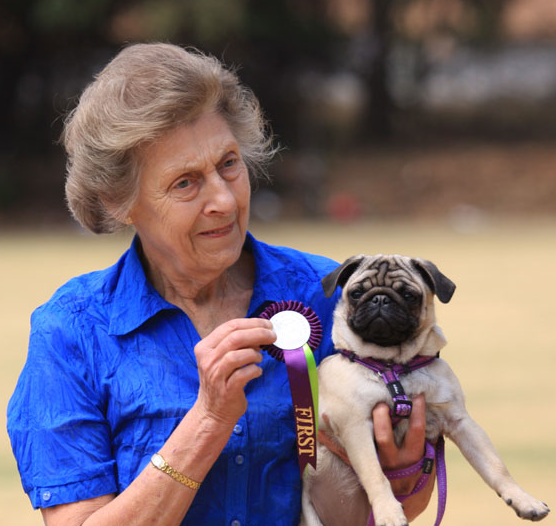
\includegraphics[
%		width=2cm,height=2cm]{pics/Diane.png}}   \\
%\end{tabular}
%
%\begin{entrylist}
%	\entry
%	{}
%	{Mathematical Science Video }
%	{ATCL, Trinity College London}
%	{\begin{shadequote}
%			Ritesh is a talented pianist who learns new repertoire quickly and has a natural sense of the required styles. He has an advanced technique and has a passion for performance.
%		\end{shadequote}}
%	\end{entrylist}
%	%------------------------------------------------
%%------------Grade 11 openday-----------------------------
%\begin{tabular}{ l }%This might not hold for long :|
%	\multirow{10}{*}{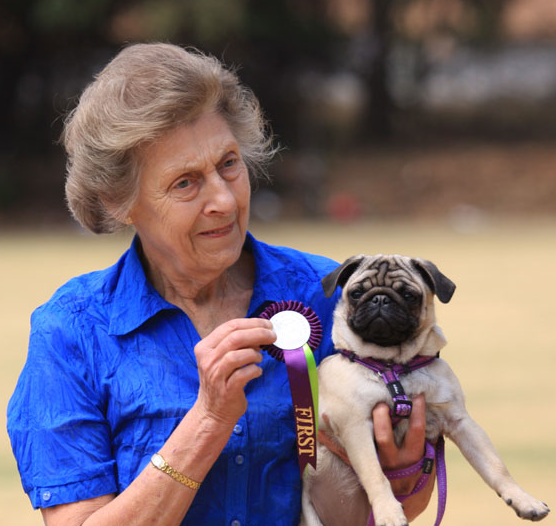
\includegraphics[
%		width=2cm,height=2cm]{pics/Diane.png}}   \\
%\end{tabular}
%
%\begin{entrylist}
%	\entry
%	{}
%	{Speaker at Grade 11 openday }
%	{ATCL, Trinity College London}
%	{\begin{shadequote}
%			Ritesh is a talented pianist who learns new repertoire quickly and has a natural sense of the required styles. He has an advanced technique and has a passion for performance.
%	\end{shadequote}}
%\end{entrylist}
%%------------------------------------------------

%\entry
%{2014}
%{Research Symposium}
%{South African Institute of Computer Science and Information Technologists}
%{Presented my Masters research on automatic music genre classification}
%%------------------------------------------------
%\entry
%{2013}
%{Research Presentation}
%{The University of the Witwatersrand}
%{Defended my research on algorithmic composition in fulfillment of my Honours degree}
%%------------------------------------------------
%\entry
%{2010}
%{Oral Presentation}
%{The University of the Witwatersrand}
%{As part of the course work for COMS4000, I presented research on how to use machines learning techniques to detect the mood of pieces of music and art}
%%------------------------------------------------
%\end{entrylist}

%----------------------------------------------------------------------------------------
%	INTERESTS SECTION
%----------------------------------------------------------------------------------------
\vspace{9}

%----------------------------------------------------------------------------------------
%	PUBLICATIONS SECTION
%----------------------------------------------------------------------------------------
%\newpage
\section{publications}
\begin{enumerate}
\item[] {\large \bf 2018}

\item[]	R. Ajoodha and B. Rosman. (2018). Advancing Intelligent Systems by Learning the Influence Structure between Partially Observed Stochastic Processes using IoT Sensor Data. Accepted in AAAI SmartIoT: AI Enhanced IoT Data Processing for Intelligent Applications, New Orleans Riverside, New Orleans, Lousiana, USA., May 2018.

\item[]	R. Ajoodha. (2018). {\it Influence Modelling and Learning between Dynamic Bayesian Networks using Score-based Structure Learning}. Ph.D. Thesis. Supervised by Dr. B. Rosman. The University of the Witwatersrand, South Africa.	
	
\item[] {\large \bf 2017}	
	
\item[]	R. Ajoodha and B. Rosman. (2017) \textit{Tracking Influence between Naïve Bayes Models using Score-Based Structure Learning.} The Pattern Recognition Association of South Africa (PRASA). IEEE accredited.

\item[]	R. Ajoodha, B. Rosman. (2017). {\it Computationally Tracking Direct Influence between Dynamic Topic Models}. Presented at the Deep Learning Indaba Symposium session. 

\item[] {\large \bf 2015}
	
\item[]	R. Ajoodha, R. Klein, B. Rosman. (2015). {\it Single-labelled Music Genre Classification using Content-based Features}. Pattern Recognition Association of South Africa, IEEE. Port Elizabeth, South Africa.
	
\item[]	R. Ajoodha. (2015). {\it Automatic Music Genre Classification}. Masters Dissertation. Supervised by Dr. B. Rosman and Dr. R Klein. The University of the Witwatersrand, South Africa.

\item[] {\large \bf 2014}

\item[]	R. Ajoodha. (2014). {\it Automatic Music Genre Classification.} Research Poster. SAICSIT M\&D Symposium: Computer Science Stream. Leriba Lodge, Centurion, South Africa.
	
\item[]	R. Ajoodha, R. Klein, M. Jakovljevic. (2014). {\it Using Statistical Models and Evolutionary Algorithms in Algorithmic Music Composition}. In Khosrow-Pour Mehdi,	editor, The Encyclopedia of Information Science and Technology, 3rd edition, IGI Global: International Publisher of Progressive Academic Research Books and Journals. Volume 10, Number doi:10.4018/978-1-4666-5888-2, pages e37893, Hershey, Pennsylvania, United States.
	
\item[] {\large \bf 2013}
	
\item[] R. Ajoodha. (2013). {\it Context-free Grammars, Gaussian Distributions and Evolutionary Algorithms in Algorithmic Music Composition.} Research Report. Supervised by Dr. R. Klein. The University of the Witwatersrand, South Africa.

\item[] {\large \bf Unpublished Manuscripts}

\item[] Ritesh Ajoodha and Benjamin Rosman. Structure Discovery of Direct Influence between Processes Represented by Hidden Markov Models (Oct 5, 2017)

\item[] Ritesh Ajoodha and Benjamin Rosman. Computationally Tracking Direct Influence between Hierarchical Dynamic Bayesian Networks using Score-based Structure Learning (July 1, 2017)

\item[] Ritesh Ajoodha and Benjamin Rosman. Structure Discovery of Direct Influence between Processes Represented by Hidden Markov Models. Manuscript to be submitted. November, 2017.

\end{enumerate}

%\section{Attended Workshops}
%\begin{enumerate}
%	\item	\textbf{Teaching Portfolio}, R. Klein, B. Rosman. (2015).	Teaching Portfolio Workshop with Ann Cameron on the 2017 06 14
%\end{enumerate}

\section{Honours, Masters, and Ph.D Supervision}
\begin{enumerate}
	
	\item[] {\large \bf 2018}
	
	\item	\textbf{Evans Molahlegi Thulare} (2018). Masters Dissertation {\it Prediction with Incomplete Data}. Data Science, University of the Witwatersrand.
	\item	\textbf{Macdeline Raesibe Mathye } (2018). Masters Dissertation. {\it An assessment of student performance at higher institutions}. Data Science, University of the Witwatersrand.
	\item	\textbf{Uvir Bhagirathi} (2018). Honours research report. {\it Automatic Venue Allocation}. Computer Science, University of the Witwatersrand.
	
	\item[] {\large \bf 2017}
	
	\item	\textbf{Vaughn Ho} (2017). Honours research report. {\it Content-based Music Recommendation Using Probabilistic Models}. Computer Science,  University of the Witwatersrand.
	\item	\textbf{Gcobisile } (2017). Honours research report. {\it Predicting the Completion of a Student's Science
		Degree based only on their First-year Marks}. Computer Science, University of the Witwatersrand.
	\item	\textbf{Jettiniel} (2017). Honours research report. {\it Automatic Labelling of Student Results as PCD, RET, MBR and MRNM}. Computer Science, University of the Witwatersrand.
\end{enumerate}

%\section{Meetings}
%\begin{enumerate}
%	\item	\textbf{Transformation committee} (2017). {\it 1.	Teaching and Learning Committee meeting}. chaired by Prof. Charis Harley. 2017/08/14, pythegorus board room.
%	
%	\item	\textbf{Transformation committee} (2017). {\it 1.	Teaching and Learning Committee meeting}. chaired  by Ann Cameron. 2017/08/14, pythegorus board room.
%\end{enumerate}

%\section{Panels}
%\begin{enumerate}
%	\item	\textbf{Isaac } (2017). {\it 1.	Teaching and Learning Committee meeting}. chaired by Prof. Charis Harley. 2017/08/14, pythegorus board room.
%	
%	\item	\textbf{Brandon Ingram } (2017). {\it Teaching and Learning Committee meeting}. chaired  by Ann Cameron. 2017/08/14, pythegorus board room.
%	
%	\item	\textbf{Yamichane Chinamale} (2017). {\it Teaching and Learning Committee meeting}. chaired  by Ann Cameron. 2017/08/14, pythegorus board room.
%\end{enumerate}

\section{Reviewed Papers}
\begin{enumerate}
	
	\item[] {\large \bf 2017}
	
	\item Unknown Authors. Efficient Bayesian Methods for Counting Processes in Partially 
	Observable Environments. 2017. AISTATS.
	
	\item Maria Bauza and Alberto Rodriguez. GP-SUM. Gaussian Processes Filtering of non-Gaussian Beliefs. Mechanical Engineering Department — Massachusetts Institute of Technology. AISTATS.
	
	\item Abdulkadir Lukman, et. al (2017). {\it Interatomic potential effect on silicon machined with diamond-a molecular dynamics study}. Submitted to PRASA. revied on 2017/10/14 (EasyChair).	
\end{enumerate}

\printbibsection{article}{article in peer-reviewed journal} % Print all articles from the bibliography

\printbibsection{book}{books} % Print all books from the bibliography

\begin{refsection} % This is a custom heading for those references marked as "inproceedings" but not containing "keyword=france"
\nocite{*}
\printbibliography[sorting=chronological, type=inproceedings, title={international peer-reviewed conferences/proceedings}, notkeyword={france}, heading=subbibliography]
\end{refsection}

\begin{refsection} % This is a custom heading for those references marked as "inproceedings" and containing "keyword=france"
\nocite{*}
\printbibliography[sorting=chronological, type=inproceedings, title={local peer-reviewed conferences/proceedings}, keyword={france}, heading=subbibliography]
\end{refsection}

\printbibsection{misc}{other publications} % Print all miscellaneous entries from the bibliography

\printbibsection{report}{research reports} % Print all research reports from the bibliography

%----------------------------------------------------------------------------------------

\end{document}